%% $Id: models.tex,v 1.20 2001/08/18 01:15:58 borning Exp $

\subsection{Models}
\label{sec:models}

The initial software implementation of UrbanSim
\citep{waddell-asce-1998} was a collection of tightly-integrated
component models, including a developer, economic and demographic
transition components, a land use component, and an external
transportation model.  The functionality of each model was
intermingled with the functionality of the others, creating a
large, complex system that did not lend itself to specialization,
refinement, or enhancement. In creating a new framework for the
UrbanSim model we sought to meet the following requirements:

\begin{itemize}
\tight
\item agent-level microsimulation of choice behavior

\item a grid-based structure to represent spatial information,
to facilitate detailed spatial queries and simulation

\item easy replacement of one model by a new version, to support system
evolution

\item easy integration of new models

\item support for different temporal and spatial scales

\item support for visualization of the model output and its processes,
for explanations and debugging

\end{itemize}

The new architecture has met these requirements.  It has also
proven relatively robust and stable, and has supported extensive
model evolution, the introduction of several additional model
components and integration with an external, concurrently-running
visualization environment \citep{pinnel-vissym-2000}.

Models represent different actors or processes in the urban
environment. In addition to encapsulating the behavior of the
actor or process, each model is also responsible for defining the
set of object types it operates on, and the fields of those
objects with which it is concerned.  A model can specify that it
wishes to share fields also declared by other models, thus
providing one technique for data-level coupling and integration of
models via the Object Store.  A model can also declare new object
types that encapsulate domain-specific data not previously
declared (e.g., a water quality model might declare a nutrient
load value).  A model may specify a set of object types and fields
it wishes to monitor for updates, creations, or deletions.  Each
model is also responsible for indicating how frequently it wishes
to be executed; there are no external constraints on how
frequently or regularly a model need run.

The design of the models is informed by research in urban
economics, sociology, civil engineering, and other disciplines.  A
discussion of the theoretical basis for the various models is
given in references
\citep{urbansim-reference-2000,waddell-env-and-planning-2000}.
A detailed specification of the models
is given in reference \citep{waddell-nse-2001}.
The present paper and \citep{waddell-nse-2001} are
complementary: the present paper concentrates on the supporting software
architecture, while the latter concentrates on the model specifications.

\subsubsection{Currently Implemented Models}

A list of the models in the current version of UrbanSim is given
below, and shown graphically in Figure \ref{fig:UrbanSim}. Each
model runs once per simulation year, unless otherwise noted.  All
of these models consist of a collection of domain-specific
case-based rules or decision rules that are encoded in Java code.
The models operate on a database consisting of individual
households, jobs, and grid cells of 150 by 150 meters containing
real estate and land.  Most of the models simulate the choices of
households, businesses and developers using discrete choice models
(multinomial logit) and Monte Carlo simulation.


\begin{figure*}
\center \resizebox{0.75
\textwidth}{!}{\includegraphics{flow2.eps}} \caption{UrbanSim
model components (source: \citep{waddell-nse-2001})}
\label{fig:UrbanSim}
\end{figure*}

\begin{description}

\item[Demographic Transition Model]
The Demographic Transition Model is responsible for modeling
births and deaths in the simulated population of households.

\item[Household Mobility Model]
The Household Mobility Model simulates the choices of households
deciding whether to move from their current residential location.

\item[Household Location Choice Model]
The Household Location Choice Model is responsible for determining
a location for each household that has no current location.

\item[Economic Transition Model]
The Economic Transition Model is responsible for modeling job
creation and loss.

\item[Employment Mobility Model]
The Employment Mobility Model determines which jobs will move from
their current locations during a particular year.

\item[Employment Location Choice Model]
The Employment Location Choice Model is responsible for
determining a location for each job that has no location.

\item[Accessibility Model]
The Accessibility Model encapsulates the interface to a (possibly
external) travel model.  It is responsible for maintaining
accessibility values for objects within each traffic analysis
zone.

\item[Land Developer Model]
The Land Developer Model simulates the action of a developer
making decisions about where and what kind of construction to
undertake (if any), including both new development and
redevelopment of existing structures.

\item[Land Price Model]
The Land Price Model simulates the evolution of land prices at
each grid cell as the characteristics of locations change over
time.

\end{description}

\subsubsection{Temporal Scale Issues and Simplifications}

UrbanSim provides a much more disaggregate and detailed simulation
than other urban land use models.  Even so, to keep the
computation manageable, the model makes many simplifying
assumptions.  For example, the Demographic Transition Model, like
most of the models, runs once per simulated year. Each simulated
year, it adjusts the total population values and distributions,
but in reality people are born and die, and move into and out of
the region, every day.  Similarly, the Land Price Model simulates
the operation of the real estate market at a temporally aggregate
level, adjusting prices once per year rather than continuously.
The software architecture has been designed to accommodate events
based on any time scale specified by a model, to allow the
integration of models with different time steps. (See
\citep{urbansim-reference-2000,waddell-queensland-2000} for
additional discussion of the theoretical basis for these design
decisions and their consequences.)

\subsubsection{Defining a Model}
\label{sec:defining-models}

The description of a model consists of a Model Definition File, and
separately, a Java class definition for the model.  The Model Definition
File includes the model's name, and the set of objects and object fields it
reads and writes, along with flags indicating if the fields are to be
shared with other models (i.e., sharing a field with an already-created
model).  Shared variables are specified explicitly in the model definition
rather than implicitly through duplicated names in order to ensure that any
duplicate use of an object field is deliberate.  This avoids a potential
problem where commonly-used names may be used in independent models but
with different semantics, and sharing the variables in that case would
cause erroneous results.  For example, one model might refer to
``population'' as a count of persons, and another as a count of households,
in which case trying to share the field would produce inconsistencies.
Information from all the relevant model definitions is combined to produce
the definitions of the objects in the Object Store (Section
\ref{sec:object-definition}).

The remainder of the model's functionality is specified by a Java class,
which must be a subclass of the abstract class \varnm{Model}.  The
following are the key methods defined by \varnm{Model}, and which are
overridden in concrete subclasses.

\begin{description}

\item[\varnm{init}] Perform any model-specific initialization, including
notifying the Model Coordinator which objects and fields it wishes to
monitor for changes.

\item[\varnm{run}] Perform the work of running the model at the current
simulated time.

\item[\varnm{nextScheduledRunTime}] Return a \keyw{float} indicating the
next simulated time that the model wishes to be run.

\item[\varnm{onCreate}] Perform any needed bookkeeping if an object of
interest has been created.  This method is invoked if one of the objects in
which this model has registered interest has been added to the Object
Store.

\item[\varnm{onChange}] An object type or field that this model monitors has
been changed---react accordingly.

\item[\varnm{onRemove}] Perform any needed bookkeeping if an object of
interest has been removed from the Object Store.

\end{description}

If the degree of interaction between a new model and existing models can be
expressed at the data level and there is a well-defined order between them
(e.g., one model's outputs are always used as inputs by another model),
then no additional information is required.  For example, the output of the
Demographic Transition Model (i.e., newly-created households that reside in
limbo) is an input to the Household Location Choice Model, and this
interaction is wholly defined at the data level (i.e., the existence of new
households in limbo).  If models need to be more tightly coupled, or
operate on differing temporal scales, the data notification interface can
be used.  For example, a continuous-time model can be set to monitor
changes to data fields it uses as inputs, and compute an updated set of
outputs only when its inputs have changed.  The Translation/Aggregation
Layer can help with models that operate on different spatial scales, for
example by aggregating from the parcel or gridcell level to the zonal
level.  The key methods used in providing this functionality are the
\varnm{onCreate}, \varnm{onChange}, and \varnm{onRemove} methods of
\varnm{Model} (as defined above), and the \varnm{postQuery} and
\varnm{postUpdate} methods of the Model Coordinator (Section
\ref{sec:TransAggrLayer}), which pass information through the
Translation/Aggregation Layer and on to the Object Store.

In addition to providing a mechanism for coupling several models using
implicit invocation, another application of the model notification
mechanism is to support the caching of frequently-accessed data within a
model, rather than repeatedly accessing it from the Object Store.  This can
be helpful if a model needs to perform costly processing on a large amount
of data, as it can compute the results once and recompute only what is
needed as parts of the underlying data are changed.  Data modification
messages serve as notification that the model's cache is no longer valid,
and supply the specific data element(s) which have changed.  For example,
the Land Price Model maintains regional and zonal-level vacancy
rates.  These more aggregate vacancy rates change slowly over time, so the
Land Price Model computes them once, and modifies them as needed as
households and employees move about the region, rather than recomputing the
aggregate vacancy rates every time the model runs.  As the vast majority of
employees and households remain where they are at each simulation step,
this approach substantially reduces the overall number and size of queries
to the Object Store.

% LocalWords:   UrbanSim logit DeveloperModel init nextScheduledRunTime Exp env
% LocalWords:  onCreate onChange onRemove gridcell gridcells postQuery noth nse
% LocalWords:  postUpdate Carlo pwaddell waddell asce pinnel vissym urbansim ne
% LocalWords:  Monte eps queensland ewly
